
\subsection{驱动因素分析}
根据气候湿润与人类活动两类驱动因素的组合,我们将黄河在历史时期的驱动因素变化过程分为六个时期(在公元400年之前,由于此时段所有原始数据的可信度均较低,我们不再后续的分析中讨论)(如表\ref{tab:ch3:periods_division})。
在过去的2000年间,研究区的大多数时期均偏干燥,包括了223次极旱年和182个洪泛年的记录。
如图\ref{fig:ch3:drivers}所示,flooding-dominant多年,累积方差的增加湿度异常显示有三个潜在的cdp,其中有两个在数据可靠的时期:晚于公元400年(CDP1 CDP2,图4 b)。没有可见的迹象人为营力在公元900年之前(图4 c)。* 900 - 1000年间农业区域向北扩大广告和* 1350 - 1650广告;第二扩张伴随着人口显著增加,而我们,因此,确认它是一种黄芪丹参滴丸(HDP1,图4 c)。我们确认第二个黄芪丹参滴丸在20世纪的人口翻了两番(HDP2,图4 c)。因此,我们细分相对于这两个历史时期cdp和两个黄芪丹参滴丸,总结如表3所示。

% Table generated by Excel2LaTeX from sheet '历史时期特征划分'
\begin{table}[htbp]
    \centering
    \caption{基于驱动因素的历史时段划分及其特点}
      \begin{tabularx}{\textwidth}{LLL}
      \toprule
      时间跨度  & 时段划分  & 主要特征 \\
      \midrule
      200BC-400AD & 数据不可信时段 & 各数据集在此时期的可信度均偏低 \\
      400-900AD & CDP1前期 & 没有明显的驱动因素 \\
      900-1100AD & CDP1时期 & 气候驱动与低水平的人类活动驱动时期 \\
      1100-1350AD & CDP1后期 & 没有明显的驱动因素 \\
      1350-1700AD & CDP2前期 & 人类活动驱动时期 \\
      1700-1900AD & CDP2时期 & 气候驱动与人类活动共同驱动时期 \\
      1900-2000AD & HDP2时期 & 人口迅速增长的人类活动强烈驱动期 \\
      \bottomrule
      \end{tabularx}%
    \label{tab:ch3:periods_division}%
\end{table}%
  

% \begin{rotate
\begin{figure}[htb]
    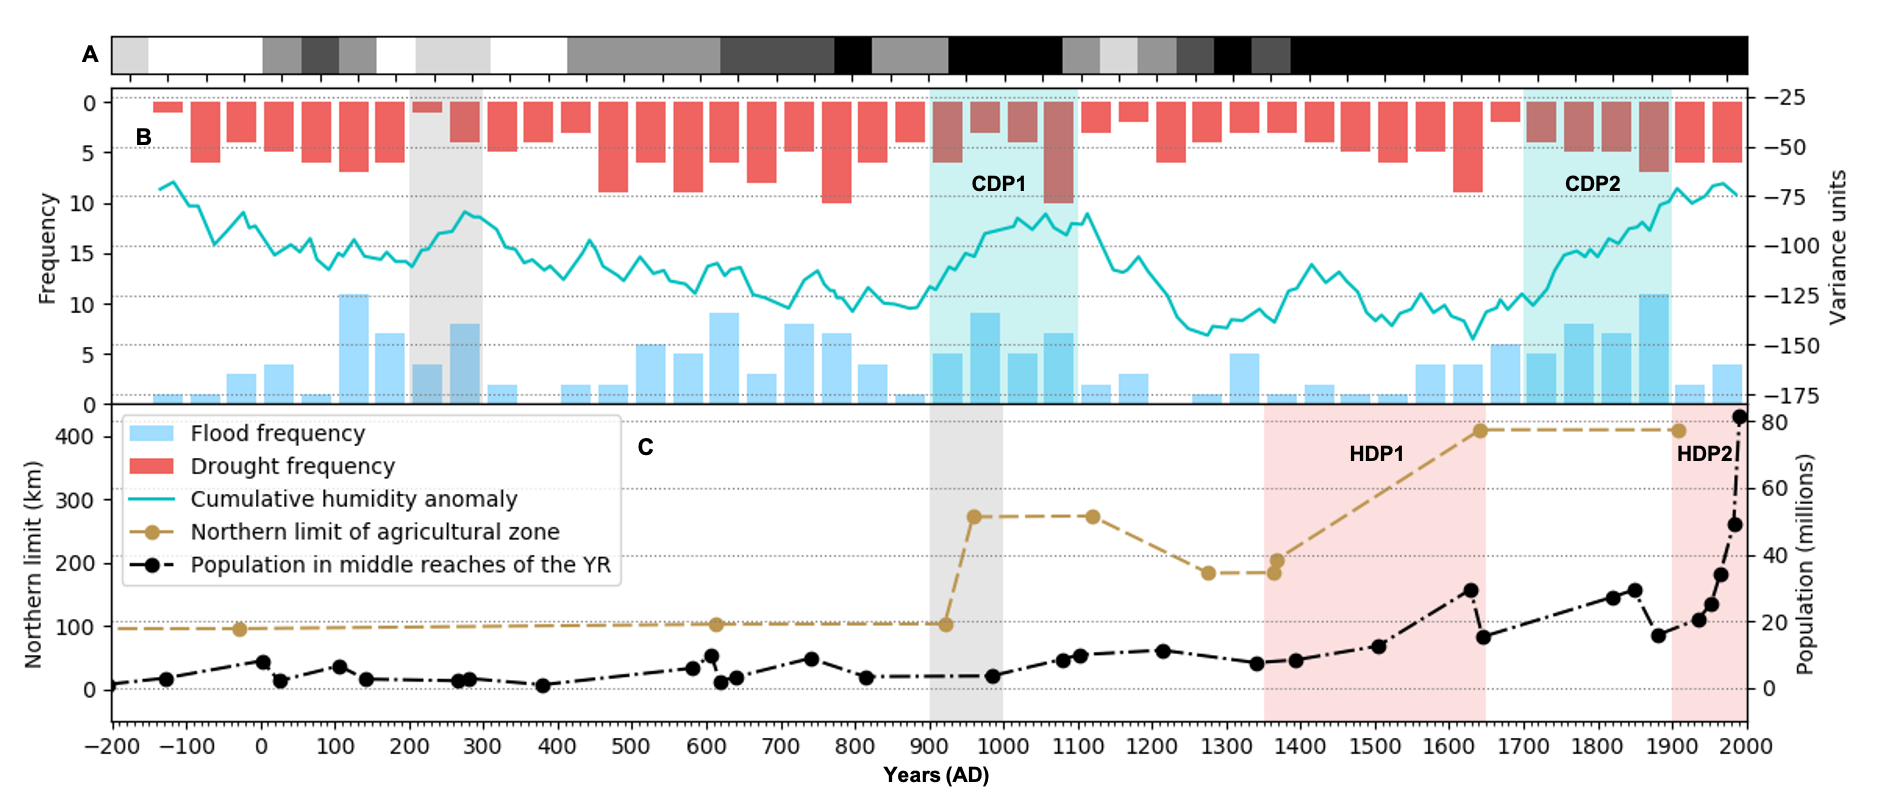
\includegraphics[width=\textwidth]{img/ch3/ch3_drivers.png}
    \caption[黄河流域历史时期稳态转换的驱动力变化]{黄河流域历史时期稳态转换的驱动力变化。
    (A) 原始数据的五级综合置信度,从极低置信度(白色)到极高置信度(黑色);
    (B) 气候驱动时期:用极端气候频率(干旱或洪水)以及累积湿润度距平共同确定的两个明显的气候驱动时段(CDPs),由蓝色阴影表示;
    (C) 人类活动驱动时期:根据黄河中游人口增长和农牧交错带北界的移动情况确定的人类活动驱动时段(HDPs),由红色阴影表示$^*$。}
    \footnotesize
    * 灰色阴影的部分表示农牧交错带北极界移动,但因缺乏可靠的人口增长证据且气候湿润也会引起农区扩张,所以不认为是一个人类活动驱动时段 HDP。
    \label{fig:ch3:drivers}
\end{figure}

\subsection{影响因素分析}
基于上述细分,溃堤的水平从偶然变成CDP1频繁,同时浏览三门山谷变得更容易(图5,CDP1)。在同一时期,它表明下游沉积速率超过4厘米/年第一次在两个样品。然而CDP1后期间,减少洪水破坏和糟糕的导航情况返回,再次,湿润的时期后,尽管没有沉积样品评估输沙量直接CDP1后(图5)。最后,当HDP1时期进入,更多的样品表现出明显的上升趋势沉积速率(图5,HDP1 HDP2)。更重要的是,最常见的洪水破坏和最糟糕的导航水平已经在这个时期。

进一步探索上述可见的变化影响,我们结合三个因素与他们的信誉对每个时期(图6)。有一些显著的差异变化的过程之前和之后的增加沙子运输上面提到的(图6中,C和D F)。首先,输沙量的最直接指标,沉积率,其可信度从HDP1依然疲弱,有可靠的增量HDP2结束后(图6 E / F)。第二,尽管这两个潮湿的cdp(图6 B和D E)推广洪水破坏,没有导航的便利在HDP2(图6 D, E),事先有变化发生在HDP1(图6 C, D)。这些表明,这两个变化过程(无花果。5和6,CDP1和HDP1 HDP2)是不同的,不管怎样。

每个时期的共同影响因素与他们的可信度。在每个半圆的图,长边的酒吧情节(扇形的半径)极坐标表示的数据,其可信度表达弧长(见2.3数据和处理)。不同颜色显示不同的影响因素:红色,黄色,蓝色,表示导航的恶化,下游沉积速率,分别和堤的洪水破坏。自相关性与径流洪水破坏和导航之间的放电是相反的,我们让他们在不同的象限,上行站输沙量高。一句话,一个更大的比率表明更高的可能性sediment-rich政权的一个特定的时期:400年-公元900年;B 900 -公元1100年;C 1100 -公元1350年;1350 - 1700 D广告;1700 - 1900 E广告;和F 1900 - 2000的广告。

\subsection{发生过程总结}
通过结合上述驱动力和影响,我们可以在千年尺度上对黄河如何进入受人类活动主导的稳态做如下解释。
